% before starting make latexindent work (preferibly do this at school)
\documentclass{article}
\usepackage{epigraph}
\usepackage{graphicx}
\title{6.033 Deep Dive 2.1 \\ UNIX FILE SYSTEM LAYERING AND NAMING}
\author{Americo De Filippo}
\begin{document}
  \maketitle
  \section{The UNIX file system}
    Unix is an operating system that is at the foundation
    of many others today, was first developed at Bell Telephone
    for the Digital Equipment Corporation PDP. Today instead
    is at the base of systems like GNU/Linux, which takes a lot
    from the standard UNIX system. Others systems like macOS are based
    on UNIX.
    \subsection{Application programming Interface for the UNIX File System}
      The UNIX file system provides an API for handling the files, the 
      user can create, choose named files, create directory, create links
      and so on... \\ But the system has they have some way to 
      organize all the files, especially those who are not created by the
      user. In the following sections we are going to have an understanding
      of the UNIX file system, moving our way up into all the layers of the
      file system. A good graphical representation is shown in the following 
      figure.
      \begin{figure}[h]
        \centering
        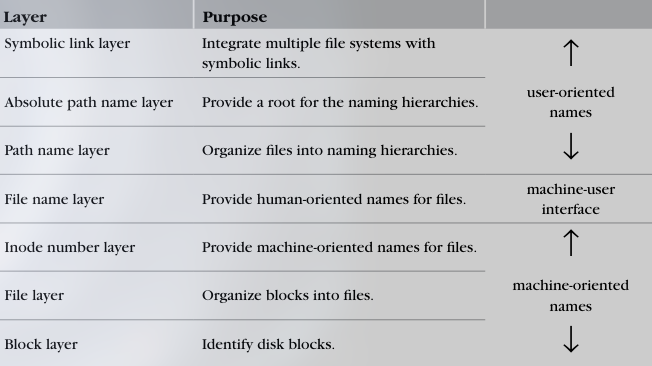
\includegraphics[width=.6\textwidth]{images/unix-layers.png}
        \caption{The Naming layers of the UNIX file system}
        \label{fig:mesh1}
      \end{figure}
    \subsection{The Block Layer}
      The block layer is the lower one and for this reason the closer to them
      machine, in fact the Block layer \textit{is} the layer which comprend the 
      physical stuff. In this layer we have the implementation of the physical
      stuff like hard drives that have to store all the \textit{durable} information
      about the system. Usually the main hard drive is organized as shown in figure 2.
      \begin{figure}[h]
        \centering
        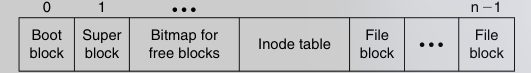
\includegraphics[width=.6\textwidth]{images/disk-layout.png}
        \caption{A simple disk layout}
        \label{fig:mesh2}
      \end{figure}
      \\ The first thing that we noticed is the naming, we have a number naming 
      for each the memory block (also called address). The first element usually is
      where are store the information for booting the operating system, in the super 
      block instead contains the size of the bitmap (for having an id of the occupied 
      and the free file blocks) and the inode table in blocks (as explained next). Another
      important feature of the hard disk is the block size. The size of the section of the 
      hard disk rapresent a problem for the operating system, because has to be made
      some trade-offs for having a good system. The usual problem could be that a small
      size can rapresent small files without wasting much memory, but could have problem
      with the handling of large size files cause has to find a lot of blocks that are 
      difficult to organize into the memory (sequential blocks). For big size blocks 
      instead the issue is with the wasting of memory that could be taken place when 
      allocation small size file in a large size block. 
    \subsection{The File Layer}
      The file layer is being implemented for handle large data that doesn't fit inside 
      a single block of the memory. A file is a ordered flow of bytes, this flow of
      data has to be stored is blocks of the memory, that are much more difficult to be
      handled for a system, for the simple reason that it has to remember which blocks 
      of the disk belongs to which file. For this reason the UNIX file system use the 
      \textit{inode}. An inode is a simple structure that stores the block numbers 
      that constitute the file and the size in bytes of the it. With this information 
      we can figure out a lot of information about the memory disposition of a single 
      file. 
    \subsection{The Inode Number Layer}
      Instead of passing table around the system we can have a compact representation
      of them, that will enable us to have a much simpler access. We will store all the 
      inodes into a table (a regular table indexed that will allow a really simple access)
      then we are going to store her at the beginning of the disk so that with these three
      layers of naming we can with a simple procedure access at the index of the block
      of a file, or have just an high level overview of the system.
    \subsection{The File Name Layer}
      For people numbers are not so friendly to be used for the purpose of naming something
      instead they are more likely to use names = strings, for making naming. But the computer
      has (for memory scopes) name files with numbers (addresses). By default, the UNIX file
      system provides the LOOKUP(filename, dir) procedure, that searches for the file (string)
      inside a directory. But what is a directory? A directory is a collection of files, and for
      the UNIX file system the \textit{inode} specify if it's a regular file or a directory.
      Usually a directory stores the map from the filename to inode numbers like that:
      \begin{figure}[h]
        \centering
        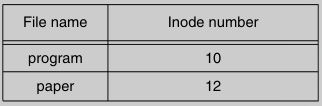
\includegraphics[width=.6\textwidth]{images/unix-directory.png}
        \caption{The graphical representation of a directory in UNIX}
        \label{fig:mesh3}
      \end{figure}
    \subsection{The Path Name Layer}
      Another useful method for organize data is the through the naming of the directory.
      In UNIX a path structure is represented like this: project/file, where project is 
      a directory with inside a file. The previous structure is called a tree of hierarchy 
      that enables us to manage our system more fully. When we want from a path access let's
      say to the block number of a file we just make a recursive function that goes to branch of our tree till it reaches the file or the directory (in this case we will
      return a map from filename to blocks numbers.
    \subsection{Links}
      The Links in a system are of fundamental importance, they allow the system to become
      much more customizable and organized. The feature that implements the link is the 
      procedure LINK(path, file), this procedure allows you to create a link between the 
      path and a file so to squash everything. The UNIX system will deny the linking of a 
      path to a directory for the possible creation of cycles like the following: LINK(a/b/c, a)
      this will create a cycle from c to a. Moreover, every inode stores a counter a reference
      to itself. In this way the deleting function could be taken place only when the counter is 
      at zero (the counter decrease with the UNLINK(path) procedure.
      \subsubsection{Soft Links}
        In Linux we can see a simple implemetation of soft link, we usually refer to them 
        as simple shortcuts to a file, in fact they preserv their own inode, because they are
        a file which points to another file in the memory but with their own inode 
      \subsubsection{Hard Links}
        Hard links on the other hand are a bit more different, when we define an Hard Link
        in UNIX we are basically creating as second pointer to a file, but despite the 
        soft side he owns the file. This concept of owning means that the file will have 
        had an increase in reference pointer, meaning that if a make an Hard link to let's
        say text.txt, then i delete text.txt, it actually still exist in the file which 
        i have made the hard link to. 
    \subsection{Renaming}
      We can implement the renaming practive via link and unlink file (here we mean Hard Links)
      the Renaming could be implemented in the following way:
      LINK(from-name, name); \\
      UNLINK(from-name); \\
      In this practive we are creating an Hard link to the file, increasing the reference
      number of 1 then we are decreasing the reference number removing the first hard link
      (which we have created when creating the file).
    \subsection{The Absolute Path Name Layer}
      At this moment we are able to create some kind of user-defined heierarcy but we are 
      able to share data or programs between users. So we need some kind of space where
      all the data are in a context which is common to all users. This space is implemented 
      before the user-name directory, this space starts with the root directory. This way
      of rappresenting the path is called absolute path, they are usueally of the 
      form: /usr/bin/..., the first folder (which in this case in usr) has a link to itself
      and if you try to perform a '..' operation you will discover that she is her own parents
      directory. A good way of viewing this is by look at this rappresentation of how we 
      are going to locate the content of a file in the memory just by knowing the path. 
      For example, to find the blocks corresponding to the file “/programs/pong.c” with 
      the information in Figure 4, we start by finding the inode table, which starts 
      at a block number (block 4 in our example) stored in the super block . From there we 
      locate the root inode (which is known to be inode number 1).  The root inode con-
      tains the block numbers that in turn contain the blocks of the root directory; in the 
      figure the root starts in block number 14. Block 14 lists the entries in the root direc-
      tory: “programs” is named by inode number 7.  The inode table says that data for inode 
      number 7 starts in block number 23, which contains the contents of the “ programs” 
      directory.  The file “pong.c” is named by inode number 9. Referring once more to the 
      inode table, to see where inode 9 is stored, we see that the data corresponding to 
      inode 9 starts in block number 61. In short, directories and files are carefully laid out 
      so that all information can be found by starting from the well-known location of the 
      root inode.
      \begin{figure}[ht]
        \centering
        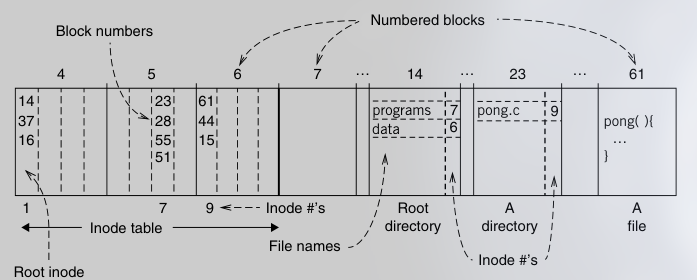
\includegraphics[width=.8\textwidth]{images/path-to-file.png}
        \caption{Memory rapprensetation of a file and hierarcy}
        \label{fig:mesh4}
      \end{figure}
    \subsection{The Symbolic Link Layer}
      The UNIX file system also enables the user to create and manage file system on others
      disks, this practice is supported by the mount and unmount commands. Let's say 
      we are mounting the /dev/df1 onto /flash, this means that all the file system of 
      the first disk in now mounted into the flash directory. Usually the mount do not
      remain after shutdowning the system.
    \subsection{Implementing the File System API}
      We others important thing to implment for make our system complete. We have seen 
      that almost all the devices are implmented via files, the basic procedure that the API
      has to provide are OPEN, READ, WRITE, CLOSE. This procedure have a lot of important 
      job, they have to provide a lot of information when using a file, like the last time
      editing, the curson block position etc... Another important aspect of the file system
      that has to do with file, are when a thread inherit a file, and he will have all 
      the current information of the process that has genereted him. Another interesting 
      proprety is the dynamic storage of the files. Usually the system stores the last used
      or most frequently used files in the cache (for memory performance) memory which is the one that he first search
      when finding a file.
\end{document}
